\section{Theoretical background} \label{Sec.TheoreticalBackground}

\subsection{Partially Observable Markov Decision Processes} \label{Sec.POMDP}

Markov Decision Processes (MDPs) are a classical formalization of sequential decision making, where actions influence not just immediate rewards, but also subsequent situations (states) and through those future rewards. Therefore, MDPs involve delayed rewards and the need to trade-off these with an immediate reward.
Partially observable Markov Decision Processes (POMDPs), which describe a more general class of problems, have one major difference, the full state is unknown. It is perceived through observations that provide only partial information about the state. A good example are Atari games used as benchmarks in this work, described in section \ref{Sec.ALE}. Individual frames often does not provide full information about the game's state which is held in the game's RAM.

In this work following definition of MDP is used: it consists of a set of hidden states $S$, a set of observations $O$ and a set of actions $A$. The dynamics of the MDP, from any state $s \in S$ and for any action $a \in A$, are determined by transition function, $P^a_{ss'} = p(S_{t+1} = s' | S_t = s, A_t = a)$, specifying the distribution over the next state $s' \in S$. A reward function, $R^a_{ss'} = p(R_{t+1} | S_t = s, A_t = a, S_{t+1} = s')$, specifies the distribution over rewards for a given state transition. Finally, as mentioned earlier, POMDP is perceived through partial observations specified via probability distribution $P_s = p(O_t | S_t = s)$. Because a state is perceived through partial observations, the state, which contains full information, is sometimes called latent or hidden.
A fixed initial state $s_0$ is assumed. In episodic MDPs, which this work considers, a sequence of states, actions and rewards form an episode which terminates with probability 1 in one of distinguished terminal states, $s_T \in S$, after finite number of transitions $T$. A return $G_t = \sum^T_{k=t+1}\gamma^{k-t-1}r_k$ is the total reward accumulated in that episode from time $t$ until reaching the terminal state at time $T$. $0 \leqslant \gamma \leqslant 1$ is a discount factor that trade-offs short-term rewards with long-term rewards.
A policy, $\pi(s, a) = p(A_T = a | S_t = s)$, maps a state $s$ to a probability distribution over actions.
A state value function, $V_\pi(s) = \EX_\pi[G_t | s_t = s]$, is the expected return from state $s$ when following policy $\pi$ where the expectation is over the distributions of the dynamics and the policy.
An action value function, $Q_\pi(s, a) = \EX_\pi[G_t | s_t = s, a_t = a]$, is the expected return after selecting action $a$ in state $s$, often called state-action pair, and then following policy $\pi$ where, again, the expectation is over the distributions of the dynamics and the policy.
Optimal state value and action value functions are unique value functions that maximise the value of every state or state-action pair, $V^*(s) = \underset{\pi}{\max}V_\pi(s), \forall_{s \in S}$ and $Q^*(s, a) = \underset{\pi}{\max}Q_\pi(s, a), \forall_{s \in S, a \in A}$. The two are related to each other by this equality: $V^*(s) = \underset{a}{\max}Q^*(s, a)$.
An optimal policy $\pi^*(s, a)$ is a policy that maximises the optimal action value function for every state in the MDP, $\pi^*(s, a) = \underset{a}{\mathrm{argmax}}Q^*(s, a)$.

Reinforcement learning assume underlying MDP or POMDP, but the dynamics, the reward function and the observations distribution are hidden from it. Consequently, these can not be used directly for planning, but one could learn them through experience. This concept is called planning and learning in literature \cite{Book.RLAI} and it is fundamental for model-based reinforcement learning.

\subsection{Reinforcement Learning} \label{Sec.RL}

Reinforcement learning (RL) is learning what to do, how to map situations to actions, so as to maximise an expected return. \cite{Book.RLAI} This mapping is called a policy $\pi$. RL consists of an agent that, in order to learn a good policy, acts in an environment, sometimes referred to as a world. The environment provides a response to each agent's action $a$ that is interpreted and fed back to the agent. The response consists of: reward $r$ that is used as a reinforcing signal and state, or observation, $s$ that is used to condition the agent's next decision. Fig.~\ref{Fig.RL} explains it in the diagram.
Each state, action, reward and next state sequence is called a step, or a transition. Multiple steps in order form a trajectory. An episode is a trajectory that starts in an initial state $s_0$ and finishes in a terminal state $s_T$. After the terminal state, the environment is reset in order to start the next episode from scratch. Very often, RL agents need dozens and dozens of episodes to gather enough experience to learn the near optimal policy. In many cases the policy is an approximation of some kind to the optimal policy and hence it will never be exactly optimal.

\begin{figure}[H]
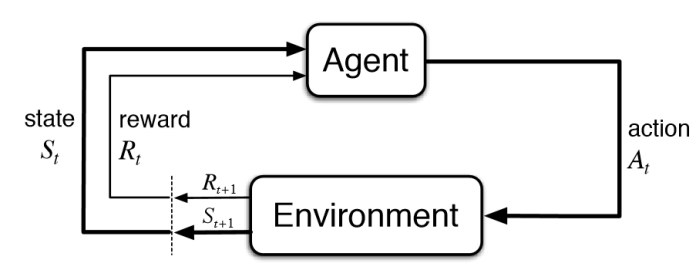
\includegraphics[]{figures/RL.jpg}
\caption[Reinforcement Learning]{Reinforcement Learning \protect\cite{Book.RLAI}}
\label{Fig.RL}
\end{figure}

Each environment can be assigned one of two characteristics from 7 categories:

\begin{itemize}
\item Fully observable vs. partially observable: If an agent have access to the complete state of the environment at each point in time, then we say that the environment is fully observable. An environment might be partially observable because of noisy and inaccurate observations or because parts of the state are simply not accessible for the agent e.g. an automated taxi cannot see what other drivers are thinking.
\item Single agent vs. multi-agent: The distinction between single-agent and multiagent environments may seem simple enough. For example, an agent solving a crossword puzzle by itself is clearly in a single-agent environment, whereas an agent playing chess is in a two-agent environment.
\item Deterministic vs. stochastic: If the next state of the environment is completely determined by the current state and the action executed by the agent, then we say the environment is deterministic. Otherwise, it is stochastic. If the environment is partially observable, however, then it could appear to be stochastic. Most real situations are so complex that it is impossible to keep track of all the unobserved aspects. For practical purposes, they must be treated as stochastic. It is often said that an environment is uncertain if it is not fully observable or not deterministic, because an agent can not be sure the outcomes of its actions.
\item Episodic vs. continuing: In an episodic environment, the agent’s experience is divided into episodes which finish at the terminal state. Crucially, the next episode does not depend on the actions taken in the previous episode. In continuing environments, on the other hand, the agent's experience may go on and on forever and there is no a distinct terminal state.
\item Static vs. dynamic: If the environment can change while an agent is deliberating, then we say the environment is dynamic for that agent. Otherwise, it is static.
\item Discrete vs. continuous: The discrete/continuous distinction applies to the internal state of the environment, to the way time is handled, and to the observations and actions of the agent. For example, the chess environment has a finite number of distinct states. Chess also has a discrete set of actions. Taxi driving is a continuous-state and continuous-time problem: the speed and location of the taxi and of the other vehicles sweep through a range of continuous values and do so smoothly over time. Taxi-driving actions are also continuous: steering angles, etc.
\item Known vs. unknown: Strictly speaking, this distinction refers not to the environment itself but to the agent’s (or designer’s) state of knowledge about the “laws of physics” of the environment. In a known environment, the outcomes, or outcome probabilities if the environment is stochastic, for all actions are given. It means that the agent have access to the environment's MDP. Obviously, if the environment is unknown, the agent will have to learn how it works in order to make good decisions.
\end{itemize}

The term dynamic programming refers to a collection of algorithms that can be used to compute optimal policies given a perfect model of the environment as a Markov decision process (MDP). Classical dynamic programming algorithms are of limited utility in reinforcement learning both because of their assumption of a perfect model and because of their great computational expense, but they are still important theoretically. Dynamic programming provides an essential foundation for the understanding of the methods presented in this thesis. In fact, all of these reinforcement learning methods can be viewed as attempts to achieve much the same effect as dynamic programming, only with less computation and without assuming a perfect model of the environment.

First question to answer is: how to compute the state value function $V(s)$ for an arbitrary policy $\pi$? The process of doing so is called policy evaluation. It is easy to note that for all states $s$: $V_\pi(s) = \EX_\pi[G_t | s_t = s] = \EX_\pi[R_{t+1} + \gamma G_{t+1} | s_t = s] = \EX_\pi[R_{t+1} + \gamma V_\pi(s_{t+1}) | s_t = s]$, where the expectations are over the environment dynamics and are subscripted by $\pi$ to indicate that they are conditional on $\pi$ being followed. The existence and uniqueness of $V_\pi$ are guaranteed as long as either $\gamma < 1$ or eventual termination is guaranteed from all states under the policy $\pi$. If the environment’s dynamics are completely known, then the equation is a system of $|S|$, number of states, simultaneous linear equations in $|S|$ unknowns. In principle, its solution is a straightforward, if tedious, computation. For more practical purposes, iterative solution methods are available \cite{Book.RLAI}, but not described here.

Major reason for computing the value function for a policy is to help find better policies. With determined the value function $V_\pi$ for an arbitrary deterministic policy $\pi$, the question now is: if for some state $s$ changing the policy to deterministically choose an action $a \neq \pi(s)$, different then from the current policy, yields higher expected return? The value function tells how good it is to follow the current policy from $s$, but would it be better or worse to change to the new policy? One way to answer this question is to consider selecting $a$ in $s$ and thereafter following the existing policy $\pi$. The value of this way of behaving is $Q_\pi(s, a) = E[R_{t+1} + \gamma V_\pi(s_{t+1}) | s_t = s, a_t = a]$, where expectation is over the environment dynamics. The key criterion is whether this is greater than or less than $V_\pi(s)$. If it is greater — that is, if it is better to select $a$ once in $s$ and thereafter follow $\pi$ than it would be to follow $\pi$ all the time — then one would expect it to be better still to select $a$ every time $s$ is encountered, and that the new policy would in fact be a better one overall. It is a natural extension to consider changes at all states and to all possible actions, selecting at each state the action that appears best according to $Q_\pi(s, a)$ and this way create a new, improved policy: $\pi' = \underset{a}{\mathrm{argmax}}Q_\pi(s, a)$. The process of making a new policy that improves on an original policy, by making it greedy with respect to the value function of the original policy, is called policy improvement. If the new policy is as good as, but not better then, the old policy, then it is the optimal policy, which can be proved without much trouble \cite{Book.RLAI}.

Policy iteration consists of two simultaneous, interacting processes, one making the value function consistent with the current policy, policy evaluation, and the other making the policy greedy with respect to the current value function, policy improvement. In policy iteration, these two processes alternate, each completing before the other begins, but this is not really necessary. In value iteration, for example, only a single iteration of policy evaluation is performed in between each policy improvement. In asynchronous dynamic programming methods, the evaluation and improvement processes are interleaved at an even finer grain. In some cases a single state is updated in one process before returning to the other. As long as both processes continue to update all states, the ultimate result is typically the same: convergence to the optimal value function and an optimal policy. \\
The term generalized policy iteration is used to refer to the general idea of letting policy-evaluation and policy-improvement processes interact, independent of the granularity and other details of the two processes. Almost all reinforcement learning methods are well described as general policy iteration. That is, all have identifiable policies and value functions, with the policy always being improved with respect to the value function and the value function always being driven toward the value function for the improvement policy, as suggested by the fig.\ref{Fig.GPI}. If both the evaluation process and the improvement process stabilize, that is, no longer produce changes, then the value function and policy must be optimal \cite{Book.RLAI}.

\begin{figure}[H]
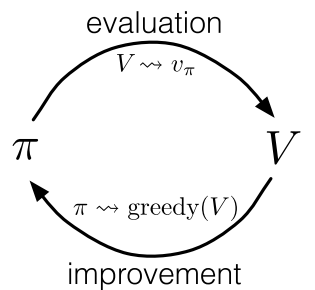
\includegraphics[width=0.4\textwidth,keepaspectratio]{figures/GPI.png}
\caption{General Policy Iteration \protect\cite{Book.RLAI}}
\label{Fig.GPI}
\end{figure}

Reinforcement learning faces two dilemmas. The first one is: How do you distribute credit for success among the many decisions that may have been involved in producing it? It is called credit-assignment problem: which past actions to reinforce for a positive outcome. \\
The second one is exploration-exploitation trade-off. To find a good policy, such that maximise an expected return, an agent needs to explore its options: if it would behave greedily all the time, it simply could not know if other actions lead to better returns. On the other hand, the agent also needs to exploit its knowledge about an environment in order to do well and progress in the environment to otherwise unavailable states. In other words, for policy evaluation to work, continual exploration needs to be assured. The most common approach to assuring that all state–action pairs are encountered is to consider only policies that are stochastic with a nonzero probability of selecting all actions in each state. \\
So called exploration policies are made to exploit an agent's knowledge about an environment, but at the same time, these constantly explore the environment's state-space. These policies are told to be soft, meaning that $\pi(a|s) > 0$ for every action in every state. One such family of policies is called $\epsilon$-greedy, meaning that most of the time they choose an action that has maximal estimated action value, but with probability $\epsilon$ they instead select an action at random. That is, all non-greedy actions are given the minimal probability of selection $\frac{\epsilon}{|A(s)|}$, where $|A(s)|$ is number of legal actions in state $s$, and the remaining bulk of the probability, $1 - \epsilon + \frac{\epsilon}{|A(s)|}$, is given to the greedy action. The bigger the $\epsilon$, the higher the exploration rate and vice versa.

There are two general approaches to reinforcement learning: on-policy methods and off-policy methods. On-policy methods attempt to evaluate or improve the policy that is used to make decisions, whereas off-policy methods evaluate or improve a policy different from that used to generate the data. In the former case, an agent is extra sensitive to imperfect updates, in cases when its value function or its policy are somehow approximated. Because the agent learns directly from its behaviour, if the bad update makes the agent behave worse then before, the agent effectively falls back in its learning progress. Also, the on-policy methods learn action values not for the optimal policy, but for a near-optimal policy that still explores, which is required as noted before. \\
An example of on-policy algorithm would be Monte-Carlo control \cite{Book.RLAI}. Because it is reinforcement learning setting an agent do not have access to underlying MDP or POMDP and needs to learn from interactions with an environment, from its experience. An obvious way to an action value function learning, or policy evaluation, is simply to play with the environment using the current policy and average the returns observed after visits to each state-action pair. It is called Monte-Carlo prediction. As more returns are observed, the average should converge to the expected value. Policy improvement is done by making the policy $\epsilon-$greedy with respect to the current value function. The two proceed according to the idea of generalized policy iteration.

In off-policy case, the behavioural exploratory policy is used for experience collection, which is then used to steadily improve the target policy towards the optimum. These methods, although favourable, are often more complex. Because the data is due to a different policy, off-policy methods are often of greater variance and are slower to converge. On the other hand, off-policy methods are more powerful and general. They include on-policy methods as the special case in which the target and behavior policies are the same. Off-policy methods also have a variety of additional uses in applications. For example, they can often be applied to learn from data generated by a conventional non-learning controller, or from a human expert. An example of off-policy algorithm would be Q-Learning \cite{Book.RLAI}, which is not described here.

There are two major kinds of reinforcement learning methods, model-free and model-based. Model-based methods rely on planning as their primary component, while model-free methods primarily rely on learning. The word planning is used in several different ways in different fields. In reinforcement learning the term is used to refer to any computational process that takes a model as input and produces or improves a policy for interacting with the modeled environment. \\
Although there are real differences between these two kinds of methods, there are also great similarities. In model-free reinforcement learning, the agent samples episodes of real experience and updates its value function from real experience, this is called learning. In model-based reinforcement learning the agent samples episodes of simulated experience and updates its value function from simulated experience, now this is planning. This symmetry between learning and planning has an important consequence: algorithms for learning can also become algorithms for planning, simply by substituting simulated experience in place of real experience.

Model-free reinforcement learning, although can be used to learn effective policies for complex tasks, typically requires very large amounts of data. In fact, substantially more than a human would need to learn the same games. How can people learn so quickly? Part of the answer may be that people can learn how the game works and predict which actions will lead to desirable outcomes. Similar mechanism is used by model-based reinforcement learning.

The model of an environment can mean anything that an agent can use to predict how the environment will respond to its actions. Given a state and an action, a model produces a prediction of the resultant next state and next reward. If the model is stochastic, then there are several possible next states and next rewards, each with some probability of occurring. Some models produce a description of all possibilities and their probabilities. These are called distribution models. Other models produce just one of the possibilities, sampled according to the probabilities. These are called sample models. The kind of model assumed in dynamic programming, estimates of the MDP’s dynamics $P^a_{ss'}$ and $R^a_{ss'}$, is a distribution model. \\
Models can be used to mimic or simulate experience. Given a starting state and action, a sample model produces a possible transition, and a distribution model generates all possible transitions weighted by their probabilities of occurring. Given a starting state and a policy, a sample model could produce an entire episode, and a distribution model could generate all possible episodes and their probabilities. In either case, it is said that the model is used to simulate the environment or rollout the trajectory and produce simulated experience. Because these models simulate the environment dynamics in order to generate transitions, they are also called dynamics models or transition models.

In artificial intelligence, there are two distinct approaches to planning according to the definition presented. State-space planning, which is viewed primarily as a search through the state-space for an optimal policy or an optimal path to a goal. Actions cause transitions from state to state, and value functions are computed over states. \\
In what is called plan-space planning, planning is instead a search through the space of plans. Operators transform one plan into another, and value functions, if any, are defined over the space of plans. Plan-space planning includes evolutionary methods.

Within a planning agent, there are at least two roles for real experience: it can be used to improve the transition model, to make it more accurately match the real environment, and it can be used to directly improve the value function and policy using the kinds of model-free reinforcement learning. The former is called model learning, and the latter is called direct reinforcement learning. The possible relationships between experience, model, values, and policy are summarized in the fig.\ref{Fig.ModelBasedRL}. It can be seen, that experience can improve value functions and policies either directly or indirectly via the transition model. This way, real experience is better utilized by using it not only once for direct reinforcement learning, but also reusing it in the future through the model. This result in better sample-efficiency over model-free methods which utilize only the direct learning path. \\
Planning is often conducted in small, incremental steps. This enables planning to be interrupted at any time, which appears to be a key requirement for efficiently intermixing planning with acting and with learning of the model. Planning in very small steps may be the most efficient approach even in pure planning problems if the problem is too large to be solved exactly or the agent can not wait for exact solution and needs to act based on approximated one.

\begin{figure}[H]
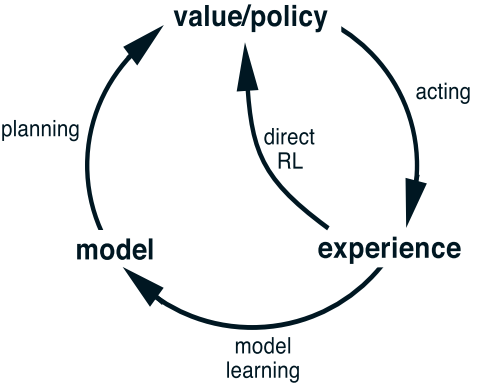
\includegraphics[width=0.4\textwidth,keepaspectratio]{figures/ModelBasedRL.png}
\caption{Model-based Reinforcement Learning. \protect\cite{Book.RLAI} Each arrow shows a relationship of influence and presumed improvement.}
\label{Fig.ModelBasedRL}
\end{figure}

\subsection{Simulation-Based Search}

Simulation-based search is something called planning at decision time \cite{Book.RLAI} and can be used in model-based reinforcement learning setting. It requires a sample model of the MDP, which can sample state transitions and rewards from $P^a_{ss'}$ and $R^a_{ss'}$ respectively. However, it is not necessary to know these probability distributions explicitly. The next state and reward could be generated by a black box simulator. The efficiency and effectiveness of simulation-based search depends in large part on the performance and accuracy of the model. The model learning problem is described later. Now, access to a perfect sample model is assumed.

Simulation-based search algorithms sample experience in sequential episodes. Each simulation begins in a root state $s_0$. At each step $u$ of simulation, an action $a_u$ is selected according to a simulation policy, and a new state $s_{u+1}$ and reward $r_{u+1}$ is generated by the sample model. This process repeats, without backtracking, until a terminal state is reached. The values of states or actions are then updated from the simulated experience. \\ Simulation-based search is usually applied online, at every time-step $t$, by initiating a new search that starts from the current state $s_0 = s_t$. The distribution of simulations then represents a probability distribution over future experience from time-step $t$ onwards. Simulation-based search exploits temporality, in other words focuses on the current situation, by learning from this specific distribution of future experience, rather than learning from the distribution of all possible experience. Furthermore, as the agent’s policy improves, the future experience distribution will become more refined. It can focus its value function on what is likely to happen next, given the improved policy, rather than learning about all possible eventualities.

Monte-Carlo simulation is a very simple simulation-based search algorithm for evaluating candidate actions from a root state $s_0$. The search proceeds by simulating complete episodes from $s_0$ until termination, using a fixed simulation policy. The action values $Q(s_0, a)$ are estimated by the mean outcome of all simulations with candidate action $a$.

Monte-Carlo tree search (MCTS) is perhaps the best-known example of a simulation-based search algorithm. It makes use of Monte-Carlo simulation to evaluate the nodes of a search tree. There is one node, $n(s)$, corresponding to every state $s$ encountered during simulation. Each node contains a total count of visits of the state, $N(s)$, a value $Q(s, a)$ and a visit count $N(s, a)$ for every possible action in a state $s$. Simulations start from the root state $s_0$, and are divided into two stages. When state $s_u$ is contained in the search tree, a tree policy selects the action with the highest value $Q(s, a)$. Otherwise, a random default policy is used to roll out simulations to completion. After each simulation, $s_0, a_0, r_1, s_1, a_1, ..., r_T$, each node $n(s_u)$ in the search tree is updated incrementally to maintain the count and mean return from that node,
$$N(s_u) \leftarrow N(s_u) + 1$$
$$N(s_u, a_u) \leftarrow N(s_u, a_u) + 1$$
$$Q(s_u, a_u) \leftarrow Q(s_u, a_u) + \frac{G_u - Q(s_u, a_u)}{N(s_u, a_u)}$$

\subsection{Deep Learning}

Machine learning gives AI systems the ability to acquire their own knowledge, by extracting patterns from raw data. It stands in opposition to classical computer programs which execute explicit instructions hand-coded by a programmer.
One example of machine learning algorithm is logistic regression. It can determine whether to recommend cesarean delivery or not \cite{Study.Cesarean}. Another widely used machine learning algorithm called naive Bayes can distinguish between legitimate and spam e-mail.

The performance of these machine learning algorithms depends heavily on the representation of the problem they are given. For example, when logistic regression is used to recommend cesarean delivery, the AI system does not examine the patient's MRI scan directly. It would not be able to make useful predictions as individual pixels in an MRI scan have negligible correlation with any complications that might occur during delivery. It, instead, gets several pieces of relevant information, such as the presence or absence of a uterine scar, from the doctor. Each piece of information included in the representation of the data is known as a feature. Logistic regression learns the relation between those features and various outcomes, such as a recommendation of cesarean delivery. The algorithm does not influence the way that the features are defined in any way.

Sometimes it can be hard to hand-craft a good problem's representation. For example, suppose that someone would like to write a program to detect cats in photographs. People know that cats are furry and have whiskers, so they might like to use the presence of a fur and whiskers as features. Unfortunately, it is difficult to describe exactly what a fur or a whisker looks like in terms of pixel values. This gets even more complicated when taking into account e.g. shadows falling on the cat or an object in the foreground obscuring part of the animal.
One solution to this problem is to use machine learning to discover not only the mapping from representation to output but also the representation itself. This approach is known as representation learning. Learned representations often result in much better performance of machine learning algorithms than can be obtained with hand-designed representations. They also allow AI systems to rapidly adapt to new tasks with minimal human intervention.

Deep learning is a particular kind of machine learning that achieves great power and flexibility by learning to represent the world as a nested hierarchy of concepts, with each concept defined in relation to simpler concepts. Deep learning solves representation learning problem by introducing representations that are expressed in terms of other, simpler representations. Fig.~\ref{Fig.DL} shows how a deep learning system can represent the concept of an image of a person by combining simpler concepts, such as corners and contours, which are in turn defined in terms of edges.

\begin{figure}[H]
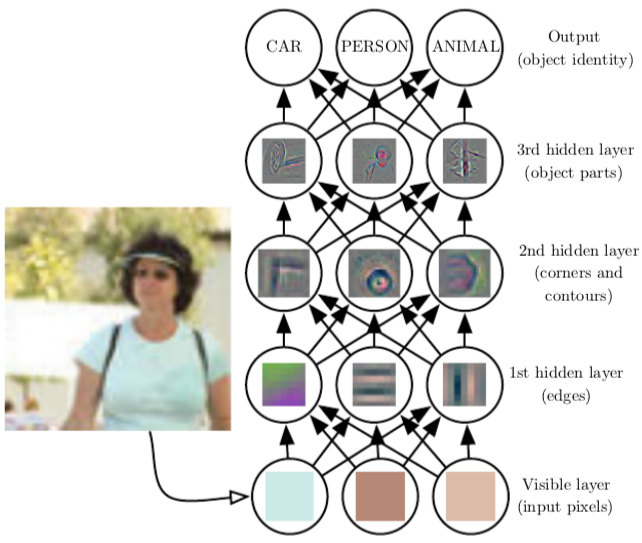
\includegraphics[width=0.8\textwidth,keepaspectratio]{figures/DL.png}
\caption[Deep Learning]{Deep Learning \protect\cite{Book.DeepLearning}}
\label{Fig.DL}
\end{figure}

The fundamental example of a deep learning model is a fully-connected (FC) neural network (NN), sometimes called a multilayer perceptron (MLP). A MLP is just a mathematical function mapping some set of input values to output values. The function is formed by composing many simpler functions, called neurons or perceptrons, into layers. Each layer provides a new representation of its input, which might be a vector, to all the neurons in the next layer by multiplying the input element-wise with its parameters and applying some kind of non-linear activation function to the sum of these products e.g. sigmoid function. Without the mentioned activation function, the multilayer NN would just simplify to a linear mapping without ability to model non-linear relationships of inputs and outputs of the NN. Fig.~\ref{Fig.MLP} shows example MLP and dependencies between perceptrons. The input is presented at the input layer. Then a hidden layer (or series of them) extracts increasingly abstract features from the image. These layers are called “hidden” because their values are not given in the data. Instead, the model must determine which concepts are useful for explaining the relationships in the observed data. Finally, this description of the input in terms of the features can be used to produce the output at the output layer.

\begin{figure}[H]
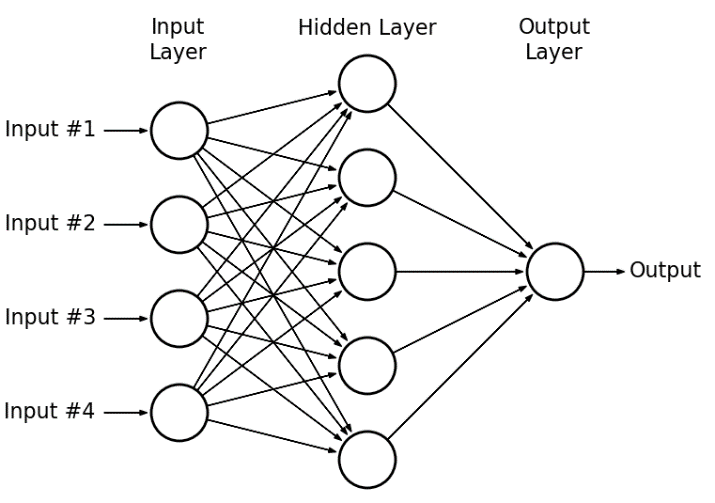
\includegraphics[width=0.8\textwidth,keepaspectratio]{figures/MLP.png}
\caption{Multilayer perceptron}
\label{Fig.MLP}
\end{figure}

Other type of very common neural network is a recurrent neural network (RNN). Humans do not start their thinking from scratch every second. As they read this thesis for example, they understand each word based on their understanding of previous words. Their thoughts have persistence. MLPs can not do this, that is why RNNs address this issue. These are networks with loops in them, allowing information to persist. In the fig.~\ref{Fig.RNN}, a chunk of neural network, $A$, looks at some input $x_t$ and outputs a value $h_t$. A loop allows information to be passed from one step of the network to the next. It turns out that RNNs are not all that different than a normal feedforward neural network. A recurrent neural network can be thought of as multiple copies of the same network, each passing a message to a successor.

\begin{figure}[H]
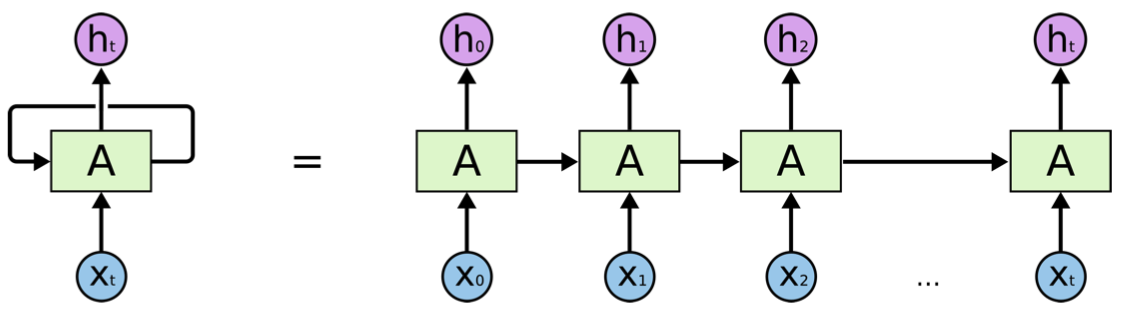
\includegraphics[width=0.8\textwidth,keepaspectratio]{figures/RNN.png}
\caption{A recurrent neural network \cite{Blog.RNNs}}
\label{Fig.RNN}
\end{figure}

Yet another very useful NN architecture is a convolutional neural network (CNN) which makes use of the fact that inputs to a NN can often have similar patterns in different parts of the input. For example in images, the object can appear in different positions in the image, but it is still the same object. CNNs exploit that fact by grouping parameters info filters in each layer and slide, or more precisely convolve, each filter across the width and height of the input volume and compute dot products between the entries of the filter and the input at any position. The 2D outputs of all filters are stacked together to form a 3D activation map. It is then processed by the next, similar, layer with its own set of filters. At the end of CNN, the final 3D volume is often flattened into a vector and then further processed by a fully-connected NN. The example CNN is shown in fig.~\ref{Fig.CNN}. \\
A CNN is able to successfully capture the spatial dependencies in an image through the application of relevant filters. The architecture performs a better fitting to the data with spatial hierarchy due to the reduction in the number of parameters involved and reusability of weights.

\begin{figure}[H]
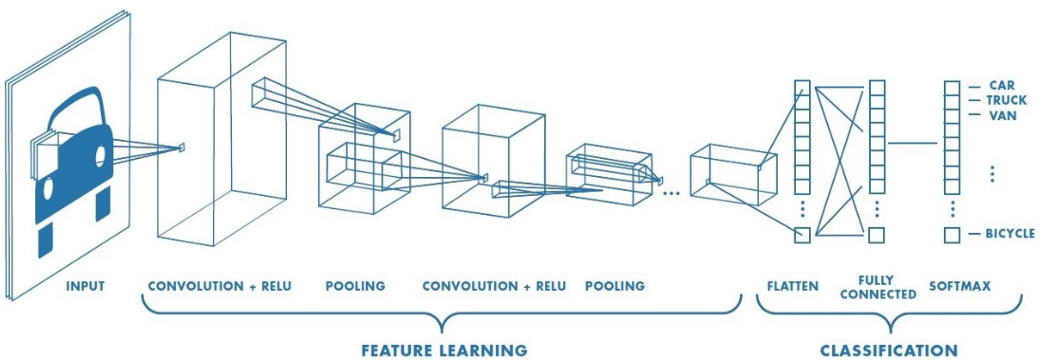
\includegraphics[width=0.9\textwidth,keepaspectratio]{figures/CNN.png}
\caption[A convolutional neural network]{A convolutional neural network \cite{Blog.CNNs}. ReLU \cite{Algo.ReLU} and Softmax are activation functions. Pooling means that each filter's output is divided into, for instance, 2 x 2 regions and only maximum value from each region is passed to the next layer.}
\label{Fig.CNN}
\end{figure}

A neural network is trained, in the simplest case, to output a correct target value for each input from a dataset. This is done by backpropagating some measure of error, how much different is the NN's output value from the target value, through the NN. This produces gradients. Gradients are vectors that point in the direction of steepest ascent of the NN's error. These are used in the opposite direction to iteratively change parameters and lower the error on the dataset. The process is repeated iteratively, updates are small steps, because gradients are first order derivatives and the directions these point in are accurate only locally. This algorithm is called gradient decent (GD) and it is at the heart of the deep learning. More about neural networks and training procedures can be found in the Deep Learning book \cite{Book.DeepLearning}.

\subsection{Model learning} \label{Sec.ModelLearning}

Generative modeling is a broad area of machine learning which deals with models of distributions $p(X)$, defined over datapoints $X$ in some potentially high-dimensional space. For instance, images are a popular kind of data for which one might create generative models. Each datapoint, which is an image, has thousands or millions of dimensions, in form of pixels, and the generative model’s job is to somehow capture the dependencies between pixels. For example, that nearby pixels have similar color, and are organized into objects. Then, one often cares about producing more examples, that are like those already in a database, using the trained generative model. \\
When training a generative model, the more complicated the dependencies between the dimensions, the more difficult the models are to train. For instance, the problem of generating images of handwritten digits from 0 to 9. If the left half of the character contains the left half of a 5, then the right half cannot contain the left half of a 0, or the character will very clearly not look like any real digit. Intuitively, it helps if the model first decides which character to generate before it assigns a value to any specific pixel. This kind of decision is formally called a latent variable or a code. That is, before the model draws anything, it first randomly samples a digit value $z$ from the set $[0, ..., 9]$, and then makes sure all the strokes match that character. It is called latent, because it is not observed, or included in the dataset, and in must be inferred in order to discover it.\\
To make this notion precise mathematically, the aim is to maximise the probability of each datapoint $X$ in the training set under the entire generative process according to: $p(X) = \int p(X|z)p(z)dz$, where $p(X|z)$ is a likelihood distribution, which generates images from latent variables, and $p(z)$ is a prior distribution, which decides on latent variables. Calculating $p(X)$ for most interesting, non-linear, models is computationally intractable. One way to bypass this is to use variational inference.

From now on, POMDP notation will be used: datapoints are now observations $o$ and latent variables are now states $s$. Variational inference can be used to train latent variable models by maximizing a lower bound of the marginal probability density $p(o) = \int p(o|s)p(s)ds$. The term $p(o|s)$ is the likelihood of the data given the latent variables $s$ and, in the case of neural networks, takes the form of a parameterised model. Instead of dealing with the prior $p(s)$ directly, variational autoencoders (VAEs) infer $p(s)$ using the posterior $p(s|o)$ \cite{Algo.VAE}. As the true form of the posterior distribution $p(s|o)$ is unknown, variational inference turns the problem of inferring latent variables into an optimisation problem by approximating the true posterior distribution with a variational distribution $q(s|o)$, called an encoder, which takes the form of a simpler distribution such as a fully factorized Gaussian, meaning the latent state vector dimensions are independent from each other, parameterised by a neural network and then minimising the Kullback-Leibler (KL) divergence between $q(s|o)$ and $p(s)$, which can be interpreted as distance between two distributions. As the KL divergence is nonnegative and minimised when $q$ is the same as $p$, the training objective for VAEs is known as the variational or evidence lower bound (ELBO) on the data log-likelihood:
$$ln p(o) \geqslant \EX_{q(s|o)}\big[ ln p(o|s) \big] - D_{KL}[q(s|o)||p(s)]$$
where $p(s)$ is very often a standard normal distribution to simplify calculations and because no prior knowledge about latent variables is assumed. The left term of ELBO is called reconstruction loss, as it makes an observation $o$ more probable given its latent variable $s$. The right term of ELBO is called regularisation loss or complexity or information bottleneck, as it pulls the approximate posterior $q$ closer to the uninformed prior $p$ and ensures this way that it explains the observation in the simplest possible way, preventing overfitting and aiding generalisation. VAEs parameters are trained using stochastic gradient descent, as common in the deep learning setting, to maximise the variational bound and this way indirectly maximise the probability of the dataset under the generative model.

Because the POMDP experience forms trajectories, where future states depend on previous states and actions, something called structured variational inference is used for model learning. The aim of this method is to train a model that accurately simulate the original environment from which the data in form of transitions was gathered. The simplest data collection approach is to use an agent that randomly explores the environment. \\
Since the random agent may not initially visit all parts of the environment, new experience needs to be iteratively collect to refine the model. It is called data-aggregation iterative method and it is often done by planning with the partially trained model.

The joint probability of states $s$, observations $o$, and rewards $r$ conditioned on the actions $a$ from the initial timestep $t = 1$ to the end of a trajectory of length $T$ is:
$$p(o_{1:T}, r_{1:T}, s_{1:T} | a_{1:T}) = p(o_1|s_1)p(s_1) \prod^T_{t=2} p(o_t|s_t)p(r_t|s_{t-1}, a_{t-1})p(s_t|s_{t−1}, a_{t−1})$$
where, besides the prior for the initial state $p(s_t)$, a transition model prior $p(s_t|s_{t−1}, a_{t−1})$ is introduced. \\
Since the model is non-linear, it is not possible to directly compute the state posteriors that are needed for parameter learning. Instead, an encoder $q(s_{1:T} | o_{1:T}, a_{1:T}) = \prod^T_{t=1} q(s_t | s_{t−1}, a_{t−1}, o_t)$ is used to infer approximate state posteriors from past observations and actions, where $q(s_t | s_{t−1}, a_{t−1}, o_t)$ could be a diagonal Gaussian with mean and variance parameterised by a neural network. Here, the filtering posterior \cite{Algo.Filtering} is used that conditions on past observations since, at the end, the model is designed to simulate future states and rewards based on past observations and actions. One may also use the full smoothing posterior during training \cite{Algo.Smoothing}, where the posterior for a single latent variable $s_t$ depends on all future observations, rewards and actions too, but it could not be used in RL setting where at each timestep the future is unknown. \\
Using the encoder, a variational bound on the data log-likelihood can be constructed. For simplicity, here only losses for predicting the observations are written, but the reward losses follow by analogy:
$$ln p(o_{1:T} | a_{1:T}) \geqslant \sum^T_{t=1} \bigg( \underset{q(s_t|o_{\leqslant t}, a_{<t})}{\EX_{} \big[ ln p(o_t|s_t) \big]} - \underset{q(s_{t-1}|o_{\leqslant t-1}, a_{<t-1})\hphantom{offset==to=====left}}{\EX \big[ D_{KL}[q(s_t|o_{\leqslant t}, a_{<t})||p(s_t|s_{t-1}, a_{t-1})] \big]} \bigg)$$
Here, the left term of ELBO is still a reconstruction loss, but now the right term of ELBO trains the approximate posterior and the transition model to be consistent with each other.

Structured variational inference rely heavily on approximation techniques. Because the final trained model is an approximation of the environment, it inducts bias that can be exploited by the agent, resulting in an agent which performs well with respect to the model, but behaves sub-optimally in the real environment \cite{Algo.WorldModels}. The approximated model can also introduce minor errors at each timestep which compound over time. The performance of planning agents can significantly suffers from these model errors \cite{Study.PlanWithImperfectModel}. Moreover, more and more inaccurate predictions over time can effectively preclude use of long, tens or hundreds of time steps, planning horizons \cite{Algo.SimPLe}.
